\documentclass[runningheads,a4paper]{llncs}

\usepackage{url}


%Example for automatically rescaling equations. 
% This is very tricky.
%\begin{equation}
%\label{eq:pimax}
%\resizebox{.55\textwidth}{!}{$
%\begin{split}
%P(\jtable_{2}|\set{E},\ttable) \propto &
%P(\keys = [jack,101],\it{Gr} = A, \it{Sat} = 1|\it{Int} = \class, \it{Rank} = 1, \it{Rat} = 3, \it{Diff}=1)\\
%\times & P(\keys = [jack,102],\it{Gr} = B, \it{Sat} = 2|\it{Int} = \class, \it{Rank} = 1, \it{Rat} = 2, \it{Diff}=2).
%\end{split}$
%}
%\end{equation}

%\usepackage{times}
%\usepackage[normaltitle,normalbib,normalmargins,normalindent]{savetrees}
\usepackage{amsmath}
\usepackage{amsfonts}
\usepackage{amssymb}
\usepackage{graphicx}
\usepackage{url}
%\usepackage{subfigure}
\usepackage{epstopdf}
\setcounter{MaxMatrixCols}{30}
%\usepackage{algorithm}
%\usepackage{algorithmic}
\usepackage{subfigure}
%\usepackage{subcaption}
\usepackage{fancyhdr}
\graphicspath{{../}{figures/}}
\usepackage{todonotes}

\DeclareMathOperator*{\argmax}{argmax}
\DeclareMathOperator*{\argmin}{argmin}
%\DeclareMathOperator{\pattern}{\pi}
\DeclareMathOperator{\Poly}{\mathbf{\mathrm{P}}}
\DeclareMathOperator{\RP}{\mathbf{\mathrm{RP}}}
%\DeclareMathOperator{\FP}{\mathbf{\mathrm{FP}}}
\DeclareMathOperator{\NP}{\mathbf{\mathrm{NP}}}
%\DeclareMathOperator{\E}{\mathbb{E}}
\renewcommand{\d}{\mathbf{d}}

\newcommand{\ZZ}{\mathbf{Z}}

\newcommand{\indep}{\ensuremath{\perp{}\!\!\!\!\!\!\!\perp{}}}
\newcommand{\dep}{\ensuremath{{\perp{}\!\!\!\!\!\!\!\not  \perp{}}}}
%\renewcommand{\L}{\mathcal{L}}
% variables denoting sets of nodes
\newcommand{\V}{V} 
\newcommand{\partC}{\mathcal{C}}
\newcommand{\pattern}{\pi}
% variables denoting nodes
\newcommand{\B}{B}
\renewcommand{\P}{P}
\newcommand{\R}{R}
\newcommand{\X}{X}
\newcommand{\Y}{Y}
\newcommand{\Z}{Z}
\newcommand{\F}{F}
\newcommand{\U}{U}
\newcommand{\W}{W}
\renewcommand{\S}{S}
\newcommand{\C}{C}
\newtheorem{mydef}{Proposition}
%variables for values
%\newcommand{\u}{u}
\renewcommand{\a}{a}
\renewcommand{\b}{b}
\newcommand{\z}{z}
\renewcommand{\v}{v}
\newcommand{\x}{x}
\newcommand{\y}{y}
\newcommand{\p}{p}
\newcommand{\s}{s}
\newcommand{\w}{w} % weights


%statistics
\newcommand{\divergence}{\it{D}}
\newcommand{\score}{\it{score}}
\newcommand{\confidence}{\it{conf}}
\newcommand{\support}{\it{support}}
\newcommand{\loglikelihood}{\it{LOG}}
\newcommand{\lof}{\it{LOF}}
\newcommand{\llmetric}{-L}
\newcommand{\lr}{\it{LR}}
\newcommand{\kl}{\it{KL}}
\newcommand{\el}{\it{EL}}
\newcommand{\mi}{\it{MI}}
\renewcommand{\mid}{\it{ELD}}
\newcommand{\jid}{\it{JID}}
\newcommand{\roc}{\it{ROC}}
\newcommand{\outrank}{\it{OutRank}}
\newcommand{\knn}{\it{KNNOutlier}}
\newcommand{\auc}{\it{AUC}}
\newcommand{\eld}{\it{ELD}}
\newcommand{\fd}{\it{FD}}
\newcommand{\parameter}{\theta}
\newcommand{\parameters}{\bs{\parameter}}
\newcommand{\bic}{\mathit{BIC}}
%random variables and graphical models
% number of values in the domain of a random variable
% variables for BNs
\newcommand{\domvals}{k}
\newcommand{\nodevalue}{\v}
\newcommand{\parvalue}{\mathbf{\pi}} % a single assignment of values to a set of 
%parents
\newcommand{\parvals}{l} % number of values of parent state.
\renewcommand{\r}{r} % CP-table row
\newcommand{\nbhd}{{\mathsf {nbdh}}}
\newcommand{\child}{\mathit{child}}
\newcommand{\parent}{\mathit{pa}}
\newcommand{\parents}{\mathbf{pa}}
\newcommand{\Parents}{\mathbf{PA}}
\newcommand{\family}{F} % families, family formulas
\newcommand{\vpi}{\mathbf{pa}} % for vectors of variable assignments
\renewcommand{\l}{\ell} % class label
\newcommand{\states}{r} % number of states of a variable
%\newcommand{\value}{value}
\newcommand{\mb}{\set{mb}} % markov blanket of a variable, vector-valued
\newcommand{\ssize}{N} % number of rows in join table; size of sample
\newcommand{\mbstates}{m} % number of states in Markov blanket
\newcommand{\frequency}{fr}
\newcommand{\pseudo}{\ast}
\newcommand{\counts}{+}
\newcommand{\weighted}{\ast}
\newcommand{\halpern}{H}
\newcommand{\Thetaa}{\theta}
\newcommand{\instance}{I}

%logic notation
%\newcommand{\predicate}{\phi}
\newcommand{\functor}{f}
\newcommand{\outdomain}{V}
\newcommand{\indomain}{\Omega}
\newcommand{\variable}{X} % first-order variable
\newcommand{\population}{\mathcal{P}}
\newcommand{\entity}{x}
\newcommand{\formula}{\phi}
\newcommand{\formulas}{\mathcal{\phi}}
\newcommand{\literal}{l}
\newcommand{\conjunction}{\set{C}} % conjunction of literals
\newcommand{\fterm}{\f} % open function term
\newcommand{\fterms}{F} % set of function terms, also nodes in JBN
\newcommand{\term}{\sigma}
\newcommand{\Terms}{\bs{\sigma}}
\newcommand{\constant}{a}
\newcommand{\constants}{\bs{\constant}}
\newcommand{\gterm}{g} % ground term
\newcommand{\gterms}{\bs{\gterm}} %list of ground terms
\newcommand{\vterm}{x} % variable term
\newcommand{\vterms}{\bs{\vterm}} % list of variable terms
\newcommand{\assign}{A} % assignment of values to Bayes net
\newcommand{\resultset}{\mathbb{R}}
\newcommand{\grounds}{\#}
\newcommand{\grounding}{\gamma}
\newcommand{\groundall}{\Gamma}
\newcommand{\vars}{\mathit{Var}} % variables in a conjunction
\newcommand{\igraph}{I} % instance-level dependency graph.
\newcommand{\assignment}{\set{a}}
\newcommand{\atom}{\ell}
\newcommand{\gnode}{\alpha}
\newcommand{\gfamily}{\ground{f}}
\newcommand{\numformulas}{m}
\newcommand{\structure}{\mathcal{S}}
% logic programs
\newcommand{\program}{\mathcal{B}}
\newcommand{\clause}{\mathcal{c}}
\newcommand{\head}{\mathit{head}}
\newcommand{\body}{\mathit{body}}
\newcommand{\crule}{\mathit{cr}} % combining rule
\newcommand{\level}{\mathit{level}} % rank of function symbols in LP

%datbase schema
\newcommand{\rcolumns}{R}
\newcommand{\ecolumns}{E}
\newcommand{\dtable}{T} % can't use \table. Generic database table
\newcommand{\datatable}{D} % generic data table, not necessarily part of database.
\newcommand{\jtable}{J} % join table
\newcommand{\Ejoin}{$J^{+}$}
\newcommand{\jtables}{m}
\newcommand{\rtable}{R} % relationship table
\newcommand{\etable}{E} % entity table.
\newcommand{\ttable}{X} % target table
\newcommand{\nextended}{n}
\newcommand{\row}{r}
\newcommand{\rows}{\mathit{rows}}
\newcommand{\col}{j}
\newcommand{\cols}{\mathit{cols}}
\newcommand{\unary}{\f} % to denote a unary or attribute function
\newcommand{\numatts}{u} % to denote the number of unary or attribute functions.
\newcommand{\g}{g} % alternative for function
\newcommand{\relational}{\mathbf{r}} % denotes a generic relational functors, can be both relationship or descriptive attribute of relationship
\newcommand{\Relation}{R} % denotes a generic boolean relation
% a special type of literal conjunction that assigns a value %to each variable
\providecommand{\keywords}{\textbf{keywords: }}
\newcommand{\loss}{\ell}
\newcommand{\class}{c} % the class attribute
\newcommand{\classlabel}{y} % the class label
\newcommand{\classifier}{\mathcal{M}}
\newcommand{\target}{t} % target object
\newcommand{\Target}{T}
\newcommand*\rfrac[2]{{}^{#1}\!/_{#2}}
\newcommand{\object}{o}
\newcommand{\Class}{C}
\newcommand{\scorediff}{\Delta}
\newcommand{\model}{B}
\newcommand{\modelprob}{\theta}
\newcommand{\profile}{P}
% the probabilities defined by a model, like conditional probabilities in a BN
\newcommand{\Targetcount}{\Gamma}
\newcommand{\neighbor}{n}
\newcommand{\feature}{V} % feature or desc attribute of object or link
\newcommand{\features}{\bs{v}} % features 
\newcommand{\Features}{\bs{V}}
\newcommand{\attribute}{a} % nonclass attribute of target object
\newcommand{\attributes}{\bs{a}}
\newcommand{\rels}{\bs{R}} % chain of relationships.
\newcommand{\maxpath}{\rho}
\newcommand{\eatts}{\it{1Nodes}}
\newcommand{\ratts}{\it{2Nodes}}
\newcommand{\atts}{\it{ANodes}}
\newcommand{\marginalize}{\it{margin}}
%special functions
\newcommand{\AVG}{\it{AVG}}
\newcommand{\instances}{n} % counts number of occurrences in DB
\newcommand{\prob}{p} % frequency of formula true in in DB

%variables denoting graphs or models
\newcommand{\mln}{M}
\newcommand{\G}{G}
\newcommand{\node}{V}
\newcommand{\nodes}{V}
\newcommand{\edges}{E}
\newcommand{\clique}{C}
\newcommand{\cliques}{\mathcal{\clique}}
\newcommand{\cliquevalue}{c}
\newcommand{\graph}{G}
\newcommand{\M}{M}
\newcommand{\J}{J}
\renewcommand{\H}{H}
\newcommand{\K}{K} % component
\renewcommand{\O}{O} % oracle
\renewcommand{\path}{\rho} % path, also foreignkey path
% Markov nets
\newcommand{\potential}{\Psi}
% database schema
\newcommand{\type}{\tau} % to denote a generic type
\newcommand{\E}{E} % for entity tables
\newcommand{\e}{e} % for specific entities
\newcommand{\f}{f}
\newcommand{\new}{\it{new}}
\renewcommand{\c}{c}
\renewcommand{\R}{R} % for relationship tables
\newcommand{\A}{A} % for attributes
\newcommand{\T}{T} % for tables generically
\newcommand{\New}{N}
\newcommand{\D}{\mathcal{D}} % for database instance
\newcommand{\databases}{\set{D}} % the number of databases
\newcommand{\vocab}{\mathcal{\L}} % for logical vocabulary associated with database
\newcommand{\name}{\mathit{name}} % generic attribute
\newcommand{\dom}{\mathit{dom}} % domain of attributes
\newcommand{\etables}{\alpha} % entity tables
\newcommand{\rtables}{\beta} % relationship table number
% specific constructs for examples


\newcommand{\team}{\it{T}}
\newcommand{\player}{\it{P}}
\newcommand{\match}{\it{M}}


\newcommand{\director}{\it{Director}}
\newcommand{\movie}{\it{Movie}}
\newcommand{\user}{\it{User}}
\newcommand{\corr}{\it{\rho}}
\newcommand{\student}{\mathit{Student}}
\newcommand{\I}{\mathit{I}}
\newcommand{\course}{\mathit{Course}}
\newcommand{\prof}{\mathit{Professor}}
\newcommand{\person}{\mathit{Person}}
\newcommand{\TA}{\mathit{TA}}
\newcommand{\actor}{\mathit{Actor}}
\newcommand{\age}{\mathit{age}}
\newcommand{\intelligence}{\mathit{intelligence}}
\newcommand{\diff}{\mathit{difficulty}}
\newcommand{\reg}{\mathit{Registered}}
\newcommand{\win}{\it{win}}
\newcommand{\ra}{\mathit{RA}}
\newcommand{\bt}{\mathit{blood type}}
\newcommand{\grade}{\mathit{grade}}
\newcommand{\gpa}{\mathit{gpa}}
\newcommand{\jack}{\mathit{Jack}}
\newcommand{\jill}{\mathit{Jill}}
\newcommand{\smith}{\mathit{Smith}}
\newcommand{\cmpt}{\mathit{CMPT120}}
\newcommand{\hi}{\mathit{Hi}}
% various constants
\newcommand{\true}{\mathit{T}}
\newcommand{\false}{\mathit{F}}
\newcommand{\normalconstant}{Z} % the normalization constant

% orderings
\newcommand{\pred}{\mathit{pred}}
%procedure names and such
\newcommand{\join}{\textsc{Join-Frequencies}}
\newcommand{\linus}{\textsc{Linus }}
\newcommand{\foil}{\textsc{Foil }}
\newcommand{\MLN}{\textsc{MLN}}
\newcommand{\treetilde}{\textsc{TILDE }}

%%%
%undirected models
\newcommand{\pot}{\phi} % potential function
%\newcommand{\theHalgorithm}{\arabic{algorithm}}
\newcommand{\test}{test}
\def\set#1{\mathbf{#1}}
\def\bs#1{\boldsymbol{#1}}
\def\ground#1{\overline{#1}}


\renewcommand{\Qconj}{\Appendterm{\FG{\TT} = \TV} {\QC}} % Use TT instead of \Ground{TI} (TI notation not defined in this paper)

\usepackage{graphicx} 


% Another view of the random regression result: if I use proportion/frequency as an aggregation function to produce an aggregate feature for propositionalization, then propositionalization is equivalent to the geometric mean as a combining rule.
% To fix the likelihood non-result about likelihood maximization, see email to Ted. Should also fix the inconsistency/incoherence problem.

\renewcommand{\marginpar}[1]{\fixneeded{(AS MARGINPAR) #1}}

\newcommand{\fixneeded}[1]{\textbf{[\footnotesize #1]}}

% Force text to appear on a separate line from a subsection header
\newcommand{\forcesubsectext}{\hskip 1pt\vskip 0pt\noindent}

% Lists in running text
% We'll probably want to regularize these later
\newcommand{\point}[1]{\noindent\emph{#1}.}
\newcommand{\subpoint}[1]{#1:}
\newcommand{\keypoint}[1]{{\em #1}}
\newcommand{\strongpoint}[1]{\paragraph{#1.}}

\newcommand{\iid}{i.i.d.}
\newcommand{\etal}{\textit{et al.}}

\graphicspath{{../../}{figures/}}

\title{Fast Learning of Relational Dependency Networks}

%\author{Oliver Schulte , Arthur E. Kirkpatrick, Yuke Zhu, Zhensong Qian \and Tianxiang Gao \\
%School of Computing Science, Simon Fraser University\\
%Vancouver-Burnaby, Canada \\
%oschulte@cs.sfu.ca}

%\author{\name Oliver Schulte \email oschulte@cs.sfu.ca \\
%       \name  Arthur E. Kirkpatrick \email ted@sfu.ca \\
%       \addr School of Computing Science, Simon Fraser University\\
%		Vancouver-Burnaby, Canada 
%       \AND
%       \name Yuke Zhu \email yukez@stanford.edu \\
%       \addr Computer Science Department, Stanford University\\
%		Stanford, California, United States 
%       \AND
%       \name Zhensong Qian \email zqian@sfu.ca \\
%       \addr School of Computing Science, Simon Fraser University\\
%		Vancouver-Burnaby, Canada 
%		\AND
%       \name Tianxiang Gao \email tgao@cs.unc.edu \\
%       \addr Department of Computer Science, University of North Carolina at Chapel Hill\\
%		Chapel Hill, North Carolina, United States 
%		    }
\author{ Oliver Schulte, Zhensong Qian, and  Arthur E. Kirkpatrick
 }

\institute{ School of Computing Science\\ Simon Fraser University\\Burnaby and Surrey, BC, Canada\\
\{oschulte,zqian,ted\}@sfu.ca\\
\url{http://www.cs.sfu.ca/~oschulte/}}                  


\date{\today}
\begin{document}

\maketitle



\begin{abstract} 
A Relational Dependency Network (RDN) is a directed graphical model widely used for multi-relational data. These networks allow cyclic dependencies, necessary to represent relational autocorrelations. We describe an approach for learning both the RDN's structure and its parameters, given an input relational database: First learn a Bayesian network (BN), then transform the Bayesian network to an RDN. Thus fast Bayes net learning can provide fast RDN learning. The BN-to-RDN transform comprises a simple, local adjustment of the Bayes net structure and a closed-form transform of the the Bayes net parameters. We empirically compare our approach to state-of-the art RDN learning methods that use functional gradient boosting. [experimental details]\end{abstract}


\section{Introduction} \label{sec:intro} Learning graphical models is one of the main approaches to extending machine learning for relational data. 
Dependency networks (DNs) \cite{Heckerman2000} are one of the major classes of graphical generative models, together with Markov networks and Bayesian networks (BNs) \cite{Pearl1988}. We describe a new approach to learning dependency networks: first learn a Bayesian network, then convert the Bayesian network to a dependency network. This hybrid approach combines the advantages of both: fast scalable learning from Bayesian networks and principled, \fixneeded{Are DNs ``principled''?  I would say that BNs are more principled, because they are consistent. The selling points of DNs are their greater generality and amenability to informal reasoning.} accurate inference from relational dependency networks. The hybrid learning algorithm produces dependency networks with accurate predictions for large complex databases, with millions of records and many predicates [how many exactly?]. 

Our main contributions are:
\begin{enumerate}
\item A faster approach for learning relational dependency networks: first learn a Bayesian network, then convert it to a dependency network.
\item A closed-form log-linear discriminative model for computing the relational dependency network parameters from Bayesian network structure and parameters.
\end{enumerate}
  
 \section{Relational Dependency Networks and Bayesian Networks} We briefly review the definition of dependency networks and their advantages for modelling relational data. 
 
 \subsection{Dependency networks and Bayesian networks} Like Bayesian networks, the structure of a dependency network is defined by a graph whose nodes are random variables and whose edges are directed. Unlike Bayesian networks, a dependency network graph may contain cycles and bi-directed edges. As with Bayesian networks, the parameters of dependency networks are conditional distributions over the value of a child node given its parents. The difference lies in the characteristic independence property of dependency networks: each node is independent of all other nodes given an assignment of values to its parents. In contrast, given an assignment of values to its Bayes net parents, there remains a dependence between a node and its children.

In graphical model terms, the parents of a node in a dependency network form a Markov blanket: The smallest set of nodes such that assigning them values will make this node independent of the rest of the network. Consequently, a parameter in a dependency network effectively specifies the probability of a node value given an assignment of values to all other nodes. Such conditional probabilities play an important role in statistical inference, for example in the widely used Gibbs sampling procedure \cite{Lunn2000}. We therefore refer to them as \defterm{Gibbs conditional probabilities}, or simply Gibbs probabilities.\footnote{In the terminology of dependency networks \cite{Heckerman2000},  Gibbs  probabilities are referred to as local probability distributions. The WinBUGS system refers to them as full conditional probabilities~\cite{Lunn2000}.}

\begin{figure}[htbp]
\begin{center}
%\resizebox{0.78\textwidth}{!}{
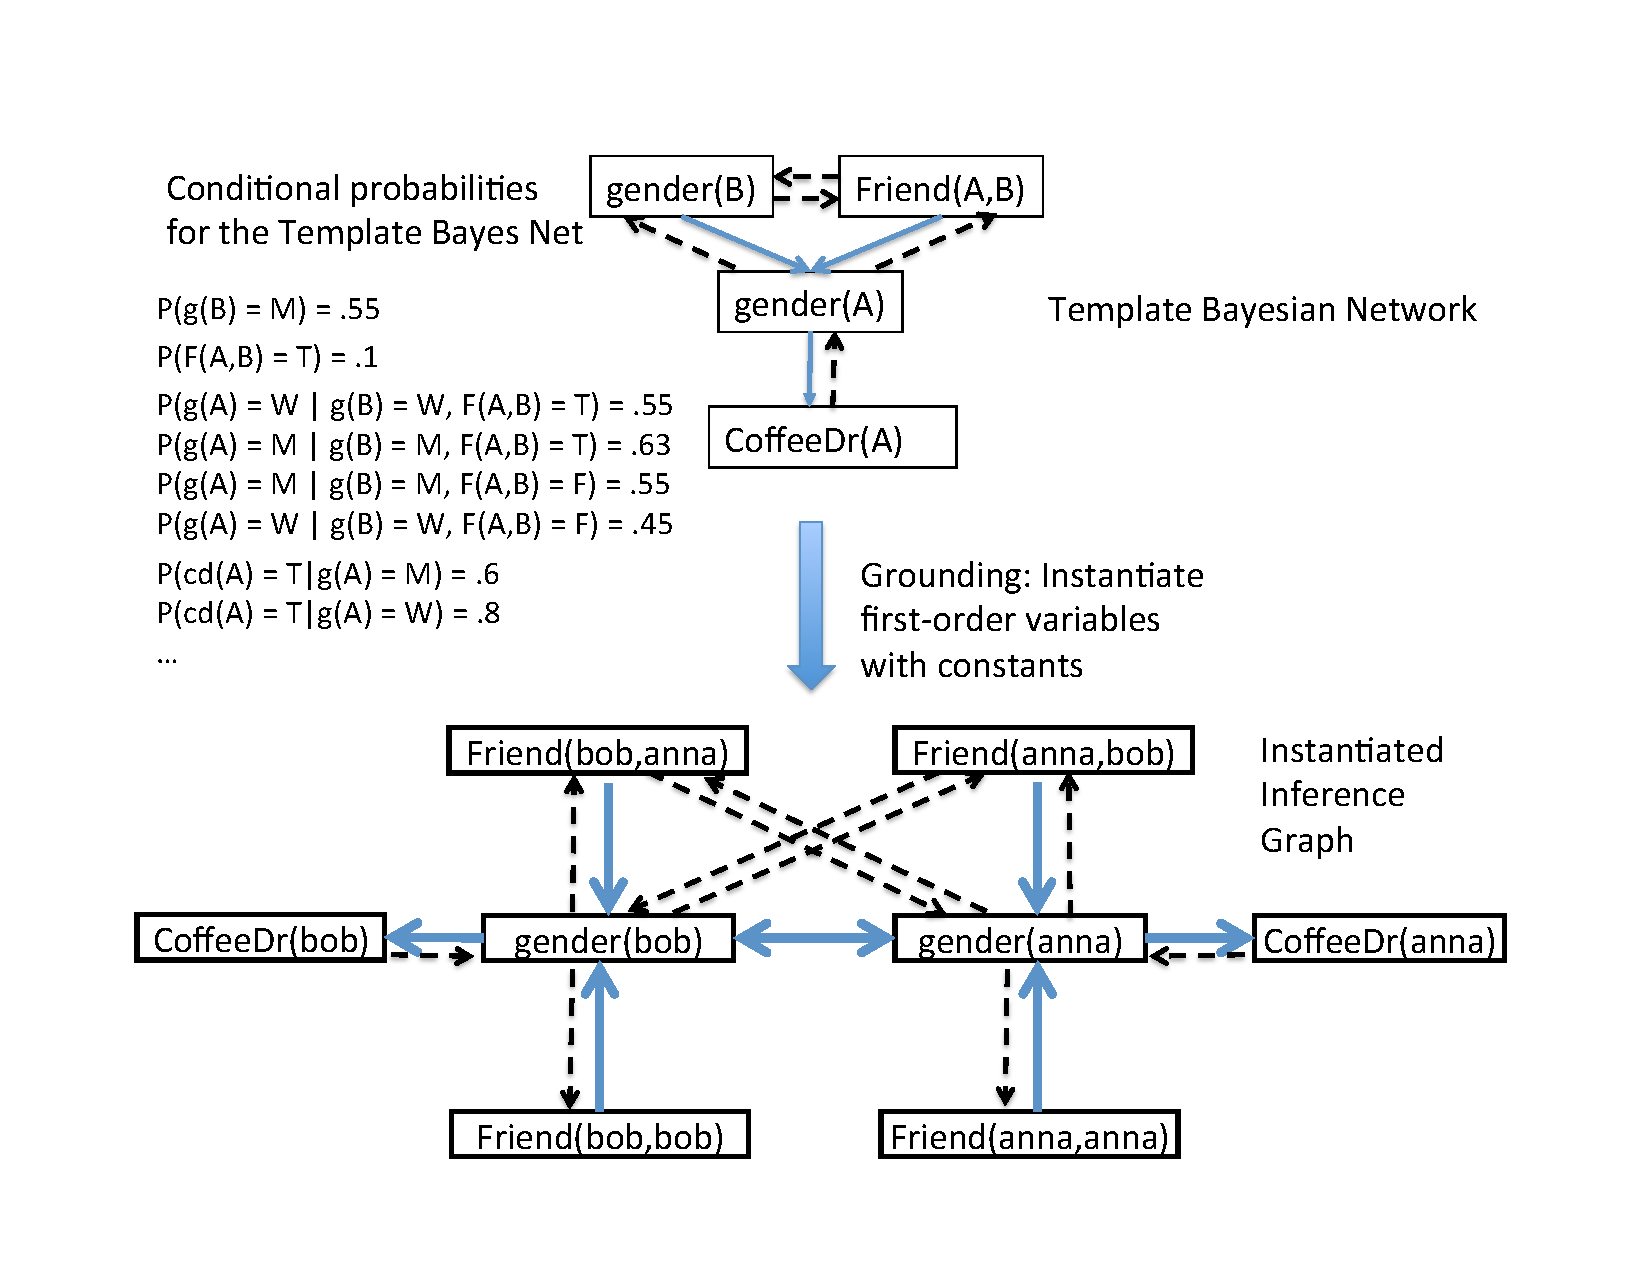
\includegraphics[width = 0.7 \textwidth]{figures/dn}
%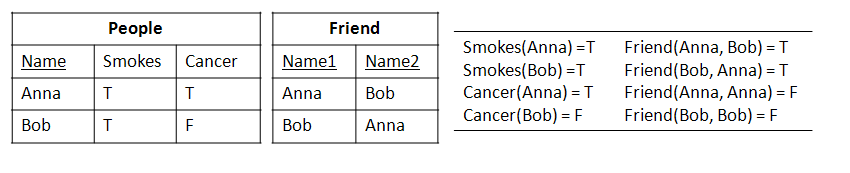
\includegraphics[width=1\textwidth]{database.png}
%}
\caption{A dependency network template model (top) and the instantiated inference graph (bottom). The Gibbs probability parameters for the inference graph specify the conditional probability of a node given its neighbors (its Markov blanket). \label{fig:dn}}
\fixneeded{Separate bidirectional links to separate links. Use different colours for links present in both BN and DN (blue) and those added for DN (black).}
\end{center}
\end{figure}

 
\subsection{Relational Dependency Networks} Relational dependency networks extend dependency networks using knowledge-based model construction (KBMC). \fixneeded{Oliver, my phrasing is likely wrong. I want to start this section with how RDNs extend DNs.} \cite{Neville2007,Natarajan2012} In this approach, a template graphical model is instantiated for a specific domain of individuals to produce an {\em  instantiated} or {\em ground} graphical model, the \defterm{inference graph} \cite{Neville2007}. Figure~\ref{fig:dn} gives a dependency network template and its grounded inference graph. An example Gibbs probability distribution for the inference graph is $$P(\it{gender}(anna)|\it{gender(bob)}, \it{CoffeeDr(anna)}, \it{Friend(anna,bob)},$$ $$\it{Friend(bob,anna)},\it{Friend(anna,anna)}).$$

Dependency network structures are well-adapted for relational data because they allow cyclic dependencies, so grounding a dependency network template is guaranteed to produce a valid dependency network.

\fixneeded{Is there anything about the next paragraph that limits it to RDNs or does it all apply to DNs? If it applies to DNs, let's move it to DN section above.}
One of the challenges for inference on relational data is that, unlike the non-relational \iid{} case, {\em a single template node may be instantiated into multiple predictors} \cite{Natarajan2008}. In the inference graph of Figure~\ref{fig:dn}, each gender of a friend of $\it{anna}$ adds one relevant predictor for the value of $\it{gender}(anna)$. The number of predictors is therefore not fixed by the model, but depends on the number of individuals related to the target individual. Relational prediction therefore requires aggregating information from different linked individuals. Two common approaches are (i) combining rules \cite{Kersting2007} and (ii) aggregation functions \cite{Getoor2007c}. In a dependency network, the aggregation encompasses the entire Markov blanket of a target node, whereas in a Bayesian network, the aggregation encompasses only its parents.
\fixneeded{Check if we still need this after full editing.}

\section{Learning Relational Dependency Networks via Bayesian Networks}

Our algorithm for rapidly learning relational dependency networks
begins with any relational learning algorithm for Bayesian networks. We then apply a simple, fast transformation of the resulting Bayesian network to a relational dependency template. Finally we apply a closed-form computation to derive the dependency network parameters from the Bayesian structure and parameters. \fixneeded{But this says nothing about the frequency computation over the database.}

Converting a Bayesian network structure to a dependency network structure is simple: for each node, add an edge pointing to the node from each member of its Bayes net Markov blanket~\cite{Heckerman2000}.  This simple means adding edges to the node from each of its children and co-parents (nodes that share a child with this one). This is equivalent to the standard moralization  method for converting a BN to an undirected model \cite[12.5.3]{Domingos2007}, \cite{Lauritzen1996}, except that the dependency network contains bi-directed edges instead of undirected edges. Bidirected edges have the advantage that they permit  assignment of different parameters to each direction, whereas undirected edges have only one parameter.
 
Converting Bayesian network parameters to dependency network parameters is simple for propositional \iid{} data: solve for the Gibbs conditional probabilities given Bayesian network parameters \cite[Ch.14.5.2]{Russell2010}. But with relational data, a value assignment for a child-parent configuration can be instantiated multiple times. \fixneeded{Why is this harder than the propositional case?} We accommodate this by using the {\em proportion of instantiations} that satisfy a child-parent value assignment as the feature function for the child-parent edge. Proportions have the desirable consequence that all feature functions are normalized to the [0,1] range. Without this normalization, features with more instantiations carry exponentially more weight. We describe the resulting equation in the next section.
\fixneeded{But this explains how proportions fix the imbalance problem, not how they fix the multi-instantiation problem.}
\fixneeded{Fit the flow diagram in if we can.}  %Figure~\ref{fig:bn-flow} shows the program flow for computing a Gibbs probability using the log-linear equation.

\fixneeded{Integration of this paper's method to previous approaches, space permitting.}

\section{The Log-Difference Frequency Equation} 
\label{sec:theequation}

\fixneeded{Do we need to justify this equation mathematically?}

We propose a log-linear equation, the \defterm{log-difference frequency equation}, for computing a Gibbs conditional probability for a ground target node, $\FG{\TT}$, given (i) a target value $\TV$ for the target node, (ii) a complete set of values $\QC$ for all ground terms other than the term of the target node, and (iii) a template Bayes net. The template structure is represented by functions that return the set of parent nodes of $\UT$, $\Pa{\UT}$, and the set of child nodes of $\UT$, $\Ch{\UT}$. The parameters of the Bayes net are
represented by the conditional probabilities of a node $\UT$ based upon its parents, $\cprob{\UT = \UV}{\Pa{\UT} = \Prange{\UT}}$.

\fixneeded{Do we need to point out how Gibbs probabilities are sufficient building block for general probabilities?}

\begin{definition}[The Log-Difference Frequency Equation]\label{def:log-diff-freq-eq}
\begin{eqnarray*}
  \Gprob{\FG{\TT} = \TV} {\QC} &\propto &  \\
 \sum_{\UT} \sum_{\UV,\Prange{\UT}}   
\qquad \left[ \ln \cprob{\UT = \UV}{\Pa{\UT} = \Prange{\UT}} \right] &
    \cdot &
    \Relfreq{\Appendterm{\UT  = \UV} {\Pa{\UT} = \Prange{\UT}}} {\Qconj}
%    \Relfreq{\Appendterm{\Ground{\UI}  = \UV} {\Ground{\Pa{\UI}} = \Prange{\UT}}} {\Qconj}
\end{eqnarray*}
where 
\begin{eqnarray*}
%\UT &\mbox{varies over} &  \TT \mbox{and its children}, \\
\UT &\mathrm{varies over} & \Setaddterm{\{\TT\}} {\Ch{\TT}}, \\
\mbox{the singleton value} \ \UV & \mbox{varies over} & \mbox{the range of}\  \UT,\\
\mbox{the vector of values} \ \Prange{\UT} & \mbox{varies over} & \mbox{the product of the ranges of} \ \UT's\ \mbox{parents}, \ \mbox{and} \\
\Relevant{\Fvar} & is & \mbox{the feature function}.
\end{eqnarray*}
\end{definition}

\fixneeded{Um, yup we need a transition here. Features and family configurations. Query conjunction.}

\subsection{Features and Feature Weights} \label{sec:features} The features are all family configurations whose child node is either the target node or a child of the target node. Thus the set of features equals the set of \defterm{query family configurations}

$$\QFC \equiv \{\Appendterm{\UI  = \UV} {\Pa{\UI} = \Prange{\UT}}: \UT \in \{\TT\} \cup \Ch{\TT}, \UV \in \Range{\UT}, \Prange{\UT} \in  \Range{\Pa{\UT}}\}.$$

For each query family configuration 
there is an associated weight $$w \equiv  \ln \cprob{\UT = \UV}{\Pa{\UT} = \Prange{\UT}}  .$$

Relations whose value is $\false$ are assigned a weight of 0.
It is well-known that eliminating irrelevant features is important for predictive accuracy in statistical-relational learning \cite{Getoor2007c,Ngo1997,Natarajan2008,Heckerman+al:SRL07}. For example, individuals whose every relationship with the target individual has value $\false$ are often irrelevant to predicting features of the target. In the example above, the gender of nonfriends (all $\B$ such that $\it{Friend}(sam, \B) = \false$) is probabilistically independent of the gender of the target. In a realistic social network, where 99\% or more of the users are {\em not} friends with a given individual, this would entail that the vast majority of groundings are irrelevant to predicting an individual's gender.


\subsection{Feature Functions} \label{sec:predictors}
For each feature, a feature function maps the query conjunction to a real number. A common feature function choice in log-linear models is the number of times that the feature is instantiated in the query conjunction. 
We use, instead, the {\em frequency} with which each feature
is instantiated in the query conjunction. 
To compute feature frequencies, we first compute feature counts, then normalize.
To count all and only instantiations that are related to the grounding of a target node, we apply the grounding to its parents, children, and co-parents.

Normalizing feature counts to obtain feature frequencies must be done with care to take account of irrelevant features. As noted above, our denominator only includes relations that have value $\true$.

\fixneeded{Define predictor here?}

\fixneeded{Introduce notation.}

\fixneeded{Is it informative to call it ``log-difference'' when there is no difference?}

\fixneeded{Target node}

\subsection{Estimating Bayes net parameers}

The Bayes net parameters can be estimated using the empirical conditional frequencies observed in an input dataset $\FG{\D}$: The parameter estimate for a family configuration is the number of instantiations of that family configuration in $\FG{\D}$, divided by the sum of all instantiation counts for that family that agree on the parent values and vary the child values. In our notation, the estimate is defined by

\newcommand{\CTPa}{\Count{\Appendterm{\TT = \TV} {\Pa{\TT} = \Prange{\TT}}}  {\FG{\D}}}
\newcommand{\CTPb}{\Count{\Appendterm{\TT = \TV'} {\Pa{\TT} = \Prange{\TT}}}  {\FG{\D}}}

\begin{equation} \label{eq:frequencies}
\estcprob{\TT = \TV} {\Pa{\TT} = \Prange{\TT}} {\FG{\D}} = 
    \frac{\CTPa}
           {\sum_{\TV' \in \Range{\TT}}\CTPb}.
\end{equation}

A theoretical justification for using the observed conditional frequencies is that these estimates maximize a pseudo-likelihood function that measures how well a template BN matches an input dataset \cite{Schulte2011,Schulte2013}. The pseudo-likelihood can be interpreted as the expected value of the log-likelihood of a random grounding of the BN nodes in the template model.

\fixneeded{Transition.}

\section{Empirical Comparison of Count vs. Proportion Feature Functions}\label{sec:empirical-comparison}

Our first set of experiments compares the predictive accuracy of the Bayes net log-linear equation \eqref{def:log-diff-freq-eq}, used with counts as feature vs. proportions. The next section describes experiments comparing the Bayes net log-linear equation with functional gradient methods for learning relational dependency networks.

\subsection{Experimental Conditions and Metrics}\label{sec:conditions}

All experiments were done on with 8GB of RAM and a single Intel Core 2 QUAD Processor Q6700 with a clock speed of 2.66GHz (there is no hyper-threading on this chip). The operating system was Linux Centos 2.6.32. Code was written in Java, JRE 1.7.0. All code and datasets are available~\cite{bib:jbnsite}. 

\subsubsection{Datasets}

We describe the datasets in terms of their representation as databases with tables. The databases follow an Entity-Relationship (E-R) design \cite{Ullman1982}. An E-R schema can be translated into our function-based logical notation as follows: Entity sets correspond to populations, descriptive attributes to functions, relationship tables to predicates, and foreign key constraints to type constraints on the arguments of relationship predicates.
%
We used %one synthetic and 
5 benchmark real-world databases from prior work~\cite{Schulte2012}. 
%The databases are fairly complex, so the experiments are computationally demanding, especially the Alchemy inference component, which needs to be applied to all groundings of all descriptive attributes to compute average predictive performance. The databases and their main characteristics are as follows. 
% and on-line sources such as \cite{bib:jbnsite}.
%In this paper we report the average result over all subdatabases in this paper and leave the evaluation of how models should evolve based on the size of data to an extension of the work in a journal paper. 


%{\em University Database.} We manually created a small dataset, based on the schema given in Table~\ref{table:university-schema}.
%The dataset is small and is used as a toy example for testing purposes. There are three entity tables, Student, Course, Professor, and 2 relationship tables RA and Registered.
%The entity tables contain 38 students, 10 courses, and 6  Professors. The $\reg$ table has 92 rows and the $\it{RA}$ table has 25 rows. %This dataset is translated into 513 ground atoms.

\begin{description}

\item[MovieLens Database] This is a standard dataset from the UC Irvine machine learning repository. 
% \cite{Schulte2012}.
%The schema for the dataset is shown in Table \ref{}.
It contains two tables representing entity sets: User with 941 tuples and Item (Movies) with 1,682 tuples.
The User table has 2 descriptive attributes, $\age$ and $\it{gender}$. We discretized the attribute $\age$ into three equal-frequency bins. The table Item represents information about the movies. It has 17 Boolean attributes that indicate the genres of a given movie. There is one relationship table Rated corresponding to a Boolean predicate. The Rated contains Rating as descriptive attribute; 80,000 ratings are recorded.  We performed a preliminary data analysis and omitted genres that have only weak correlations with the rating or user attributes, leaving a total of three genres (Drama, Horror, Action).
%
%The full dataset contains 170,143 ground atoms and is too big for Alchemy to perform learning. We made small subsamples to make the experiments feasible. Subsampling 100 Users and 100 Items transforms to an Alchemy input file with 3,485 ground atoms. Structure learning with Alchemy takes around 30 min.
%Subsampling 300 Users and 300 Items transforms to an Alchemy input file with 27,134 ground atoms. Structure learning with Alchemy takes about 2 days to run.
%The full table with 100,000 ratings exceeded the memory limits of Tetrad, so we randomly picked 40\% of the ratings of the relationship table as input data.

\item[Mutagenesis Database] This dataset is widely used in Inductive Logic Programming research \cite{Srinivasan1996}. %It contains 4 tables total to 15218 tuples. 
We used a previous discretization \cite{Schulte2012}.
Mutagenesis has two entity tables, Atom with 3 descriptive attributes, and Mole (decribing molecules), with 5 descriptive attributes. 
%including two attributes that are discretized into ten values each (logp and lumo).
There are two relationship tables, MoleAtom, indicating which atoms are parts of which molecules, and Bond, which relates two atoms and has 1 descriptive attribute. 
%The full dataset, with 35,973 ground atoms, crashed Alchemy with both structure  and parameter learning. A subsample with 5,017 ground atoms did not terminate for structure learning, but weight learning was feasible. The computational difficulties of Alchemy compared to the MovieLens dataset are  due to the high number of descriptive attributes.
%%another subsample with
%Representing a relationship between entities from the same table in a parametrized Bayes net requires using two or more variables associated with the same population (e.g., $\it{Bond}(\A_{1},\A_{2}))$.
%(Techreport 2009) describes a straightforward extension of Algorithm~\ref{alg:structure} for this case, which we applied to the Mutagenesis dataset.\footnote{Reference omitted for blind review.}
%We also tested our method on the Financial dataset with similar results, but omit a discussion due to space constraints.

\item[Hepatitis Database] This data is a modified version of the PKDD02 Discovery Challenge database \cite{Frank2007}. %, which includes removing tests with null values. 
The database contains information on laboratory examinations of 771 hepatitis B- and C-infected patients, taken
between 1982 and 2001. The data are organized in 7 tables (4 entity tables,  3 relationship tables) with 16 descriptive attributes. They contain basic information about the patients, results of biopsy, information on interferon therapy, results of out-hospital examinations, and results of in-hospital examinations. 

\item[Mondial Database] 
%
%\textbf{Hassan: which version did you use? The full one from http://www.dbis.informatik.uni-goettingen.de/Mondial/mondial-ER.pdf or Bahareh's?} 
%
This dataset contains data from multiple geographical web data sources. 
%Our dataset contains 4 entity tables, $\it{Country},\it{Continent},\it{Economy},\it{Government}$, where the latter three are related to Country by many-one relationships, and one relationship table $\it{Borders}$ that relates two countries.
%This dataset contains data from multiple geographical Web data sources \cite{mondial}. 
We follow the modification of She~\etal~\cite{wangMondial}, and use a subset of the tables and disretized features: 2 entity tables, $\it{Country},\it{Economy}$. The descriptive attributes of Country are continent, government, percentage, majority religion, population size. The descriptive attributes of Economy are inflation, gdp, service, agriculture, industry. A relationship table Economy\_Country specifies which country has what type of economy. A self-relationship table Borders relates two countries.
  %$\it{Country},\it{Continent},\it{Economy},\it{Government}$, where the latter three are related to Country by many-one relationships, and one relationship table $\it{Borders}$ that relates two countries. Our dataset includes a self-relationship table Borders that relates two countries.



\item[UW-CSE database] This dataset lists facts about the Department of Computer Science and Engineering at the University of Washington, such as entities (e.g., $Person$, $Course$) and the relationships (i.e. $AdvisedBy$, $TaughtBy$).
% \cite{Domingos2007}. 
%The total number of ground atoms is 4,106,841. The database contained a total of 3380 ground atoms. 

\end{description}

\subsubsection{Prediction Metrics}
We evaluate the algorithms using classification
accuracy and conditional log likelihood (CLL). These metrics have been used in previous evaluations of MLN learning~\cite{Domingos2007,Schulte2012}.  For each fact $\FG{\TI} = \TV$ in the test dataset, we evaluate the accuracy of the predicted Gibbs probability $\Gprob{\FG{\TI} = \TV} {\QCtarget}$, where $\QCtarget$ is a complete conjunction for all ground terms other than $\FG{\TI}$. Thus $\QCtarget$ represents the values of the input variables as specified by the test dataset.
For classification accuracy, a model's prediction is scored as correct if the true value of the ground term in the test dataset receives the highest Gibbs probability. 
CLL is the average of the logarithm of the Gibbs probability for each fact in the test dataset. Thus $\exp(CLL)$ is the geometric mean of the Gibbs probabilities.\footnote{The geometric mean of a list of numbers $x_{1},\ldots,x_{n}$ is $(\prod_{i} x_{i})^{1/n}$.}
Both metrics are reported as averages over all functors that represent descriptive attributes. For binary predicates we also use Area Under Curve, computed as in \marginpar{fill in reference}.
The learning methods were evaluated using 5-fold cross-validation. Each database was split into 5 folds by randomly selecting entities from each entity table, and restricting the relationship tuples in each fold to those involving only the selected entities  (i.e., subgraph sampling~\cite{Frank1977,Schulte2012}). The models were trained on 4 of the 5 folds, then tested on the remaining one. All results are averages from 5-fold cross validation, over all descriptive attributes in the database. 


\subsubsection{Learning the Bayes Net Structure and Parameters}

All the methods compared in this experiment require a prior Bayes net structure and parameters.
To obtain the structure, the learn-and-join algorithm~\cite{Schulte2012} was applied to each benchmark database. The parameters were computed from the empirical conditional frequencies in the database (Eq.~\ref{eq:frequencies}) using previously-published algorithms~\cite{Schulte2013}. The resulting structure and parameters were used for all methods in this experiment. 
 


\subsection{Results} 

Table~\ref{table:bn} summarizes the results for the Bayes net log-linear model.
The numbers represent an average over many individual scores, one for each fact
%ground literal 
in the database. 
For instance in the biggest dataset, MovieLens, the average is over a total of 170,000 scores; see Table~\ref{table:learn-times}. 

To aid interpretability, we also report the following transformation of CLL: prob. ratio = $\exp(CLL(proportion) - CLL( count))$. This quantity represents the geometric mean, over all test facts, of the fact likelihood ratio of the $\it{proportion}$ feature function over the $\it{count}$ feature function.
For instance, the value of 1.06 for the dataset UW means that on (geometric) average, the likelihood that the $\it{proportion}$ feature function assigns to the correct value for the target node is 1.06 times that assigned by the the $\it{count}$ feature function.


 
\begin{table}[thbp]
\caption{Conditional log-likelihood (log-probabilities) and classification accuracy (in percent) of Bayesian network log-linear equations. We show averages and standard deviations. The probability ratios can be interpreted as the geometric average ratio of likelihoods assigned by the count resp. proportion feature functions to the true target node value.}

%\resizebox{0.5\textwidth}{!}{

\begin{center}
%\resizebox{0.5\textwidth}{!}{
\begin{tabular}{|l|c|c|c|c|c|}
\hline
Accuracy& UW & Mondial & MovieLens & Mutagenesis & Hepatitis \\\hline
 count & 78 $\pm$ 0.08 & 40 $\pm$ 0.05 & 64 $\pm$ 0.01 & 62 $\pm$ 0.05 & 49 $\pm$ 0.03 \\

proportion & \textbf{81} $\pm$ 0.06 & \textbf{45} $\pm$ 0.04 & \textbf{65} $\pm$ 0.01 & \textbf{67} $\pm$ 0.03 & \textbf{55} $\pm$ 0.02 \\
\hline
\end{tabular}
\end{center}

\begin{center}
\begin{tabular}{|l|c|c|c|c|c|}
\hline
CLL & UW & Mondial & MovieLens & Mutagenesis & Hepatitis \\\hline
count & -0.47 $\pm$ 0.10 & -1.47 $\pm$ 0.17 & -1.19 $\pm$ 0.07 & -0.84 $\pm$ 0.03 & -1.33 $\pm$ 0.07 \\
proportion & \textbf{-0.41} $\pm$ 0.04 & \textbf{-1.34} $\pm$ 0.09 & \textbf{-0.71} $\pm$ 0.01 & \textbf{-0.73} $\pm$ 0.04 & \textbf{-1.07} $\pm$ 0.10\\
Prob. ratio & 1.06 & 1.14 & 1.62 & 1.12 & 1.30\\
\hline
\end{tabular}
%}
\end{center}
\label{table:bn}
\end{table}%

Using proportions rather than counts improves the conditional log-likelihood score, substantially on MovieLens and Hepatitis (probability ratio 1.62 resp. 1.30).
Proportions also achieve top performance for  classification accuracy. However, the classification score difference between proportions and counts is small ($<1\%$), except for a bigger improvement (3\%) on MovieLens. Whereas classification accuracy is a 0-1 loss function, CLL is continuous, so balancing factors with proportions has substantially more impact on CLL. In sum:\keypoint{Using Bayes net parameters, proportion feature functions outperform count feature functions.} This finding supports our hypothesis that using proportions as feature functions is an effective way of addressing the imbalance problem.



\section{Comparison with RDN-Boost}
\label{sec:general-weights}

The experiments in Section~\ref{sec:empirical-comparison} held the Bayes net structure and parameters constant and compared transformations of the BN parameters into log-linear weights. In this section we examine a setting where the same features are computed from the BN structure, but weights are {\em not} computed from the BN parameters. Instead weight values are optimized by a local search method. This experiment used the same conditions and metrics described in Section~\ref{sec:conditions}.  In addition to comparing predictive performance, we also report learning times.

To learn the weights, we applied the default training procedure of the Alchemy package \cite{Kok2009a}.  This procedure takes as input a set of features specified as logical formulas, and returns a weight for each formula. We followed the method recommended by the Alchemy group \cite{bib:bayes-convert} for converting a Bayes net structure to a Markov Logic Network structure: For each family configuration $\family_{ijk}$ in the BN, add a conjunction of literals that specifies the state. We also added unit clauses for each node-value combination, as recommended by the Alchemy group; unit clause weights can represent the bias weight of a log-linear equation.


%The Markov Logic Network (MLN) structure for weight learning was computed by the moralization procedure \cite[12.5.3]{Domingos2007}: convert a parametrized Bayes net to an MLN structure that contains,  for each family state $\family_{ijk}$ in the net, a conjunction of literals that specifies the state. This is the recommended procedure%~\cite{bib:bayes-convert} for converting a Bayes net to a Markov Logic Network.\footnote{We also added unit clauses for each node-value combination, as recommended by the Alchemy group.}  
%; see also Section~\ref{sec:other}. Weights learned by Alchemy are therefore appropriate for count regression. 
We refer to moralization+weight learning as the \defterm{MBN} method, for ``Moralized Bayes Net''   \cite{Khosravi2010}. 
MBN has been the state-of-the-art method for log-linear prediction with Bayes nets \cite{Schulte2012}.
Markov Logic Network weight learning optimizes for log-linear inference with counts as feature functions~\cite{Schulte2011}. The prediction probabilities were computed exactly using the log-linear equation with counts as feature functions. We used an exact computation rather than approximate inference
(e.g., MC-SAT), to avoid confounding the effect of the log-linear equation with that of inference implementation. Experiments with MC-SAT produced similar results. We also computed the results with frequencies as feature functions, which for optimized weights were very similar, so we do not present them. 





\subsection{Results}

\keypoint{The Bayes net frequency regression predictions are competitive with those from a model with optimized general weights.}

%%UW values are from Zhensong
\point{Accuracy} Table~\ref{table:mbn} shows the scores of the MBN method, together with the log-difference frequency results from Table~\ref{table:bn}. The log-difference frequency model scores slightly higher than the MBN weights on every dataset, with the biggest differences on Mutagenesis (5\%),  MovieLens (5\%) and Hepatitis (4\%). 

\begin{table}[thbp]

\caption{Conditional log-likelihood (log-probabilities) and classification accuracy (percent) of MBN and log-difference frequency predictions.}

\begin{center}

\begin{tabular}{|l|c|c|c|c|c|}
\hline
Accuracy& UW & Mondial & MovieLens & Mutagenesis & Hepatitis \\\hline
MBN & 80 $\pm$ 0.05 & 44 $\pm$ 0.04 & 60 $\pm$ 0.02 & 62 $\pm$ 0.02 & 51 $\pm$ 0.02 \\\hline
log-diff $+$ freq & \textbf{81} $\pm$ 0.06 & \textbf{45} $\pm$ 0.04 & \textbf{65} $\pm$ 0.03 & \textbf{67} $\pm$ 0.03 & \textbf{55} $\pm$ 0.02 \\
\hline
\end{tabular}
\end{center}


\begin{center}
\begin{tabular}{|l|c|c|c|c|c|}
\hline
CLL & UW & Mondial & MovieLens & Mutagenesis & Hepatitis \\\hline
MBN & -0.44 $\pm$ 0.07 & \textbf{-1.28} $\pm$ 0.07 & -0.79 $\pm$ 0.03 & -0.91 $\pm$ 0.09 & -1.18 $\pm$ 0.26 \\
log-diff $+$ freq & \textbf{-0.41} $\pm$ 0.04 & -1.34 $\pm$ 0.09 & \textbf{-0.71} $\pm$ 0.01 & \textbf{-0.73} $\pm$ 0.04 & \textbf{-1.07} $\pm$ 0.10 \\
Prob. ratio & 1.03 & 0.94 & 1.08 & 1.20 & 1.12\\
\hline
\end{tabular}
%}
\end{center}
\label{table:mbn}

\end{table}%


\point{CLL}
The log-difference frequency  model scores better than MBN model on UW, MovieLens, Mutagenesis and Hepatitis (probabilities 3--20\% higher) and scores slightly worse on Mondial (6\% lower probability); see Figure~\ref{fig:summarize}.

\begin{figure}[htbp]

\begin{center}
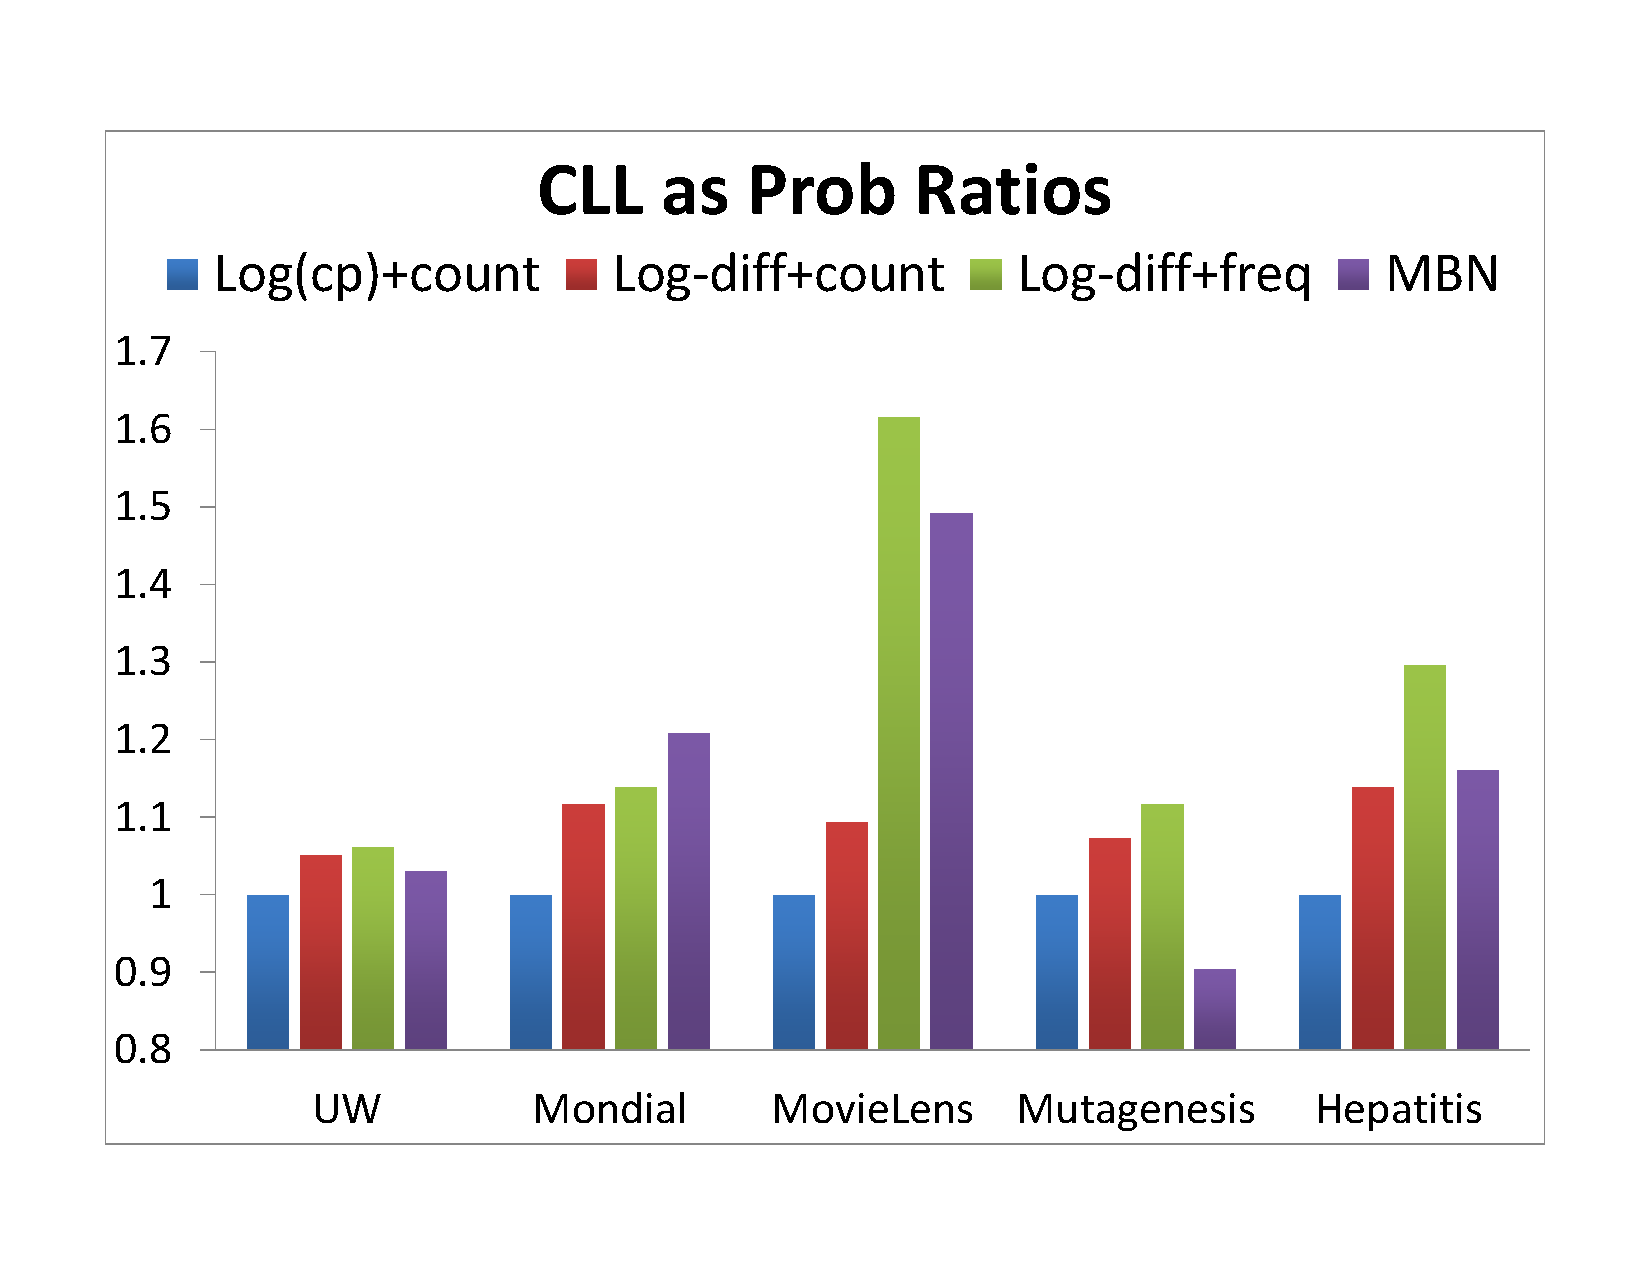
\includegraphics[width=0.6\textwidth]{CLL_Prob_Ratios_New}
%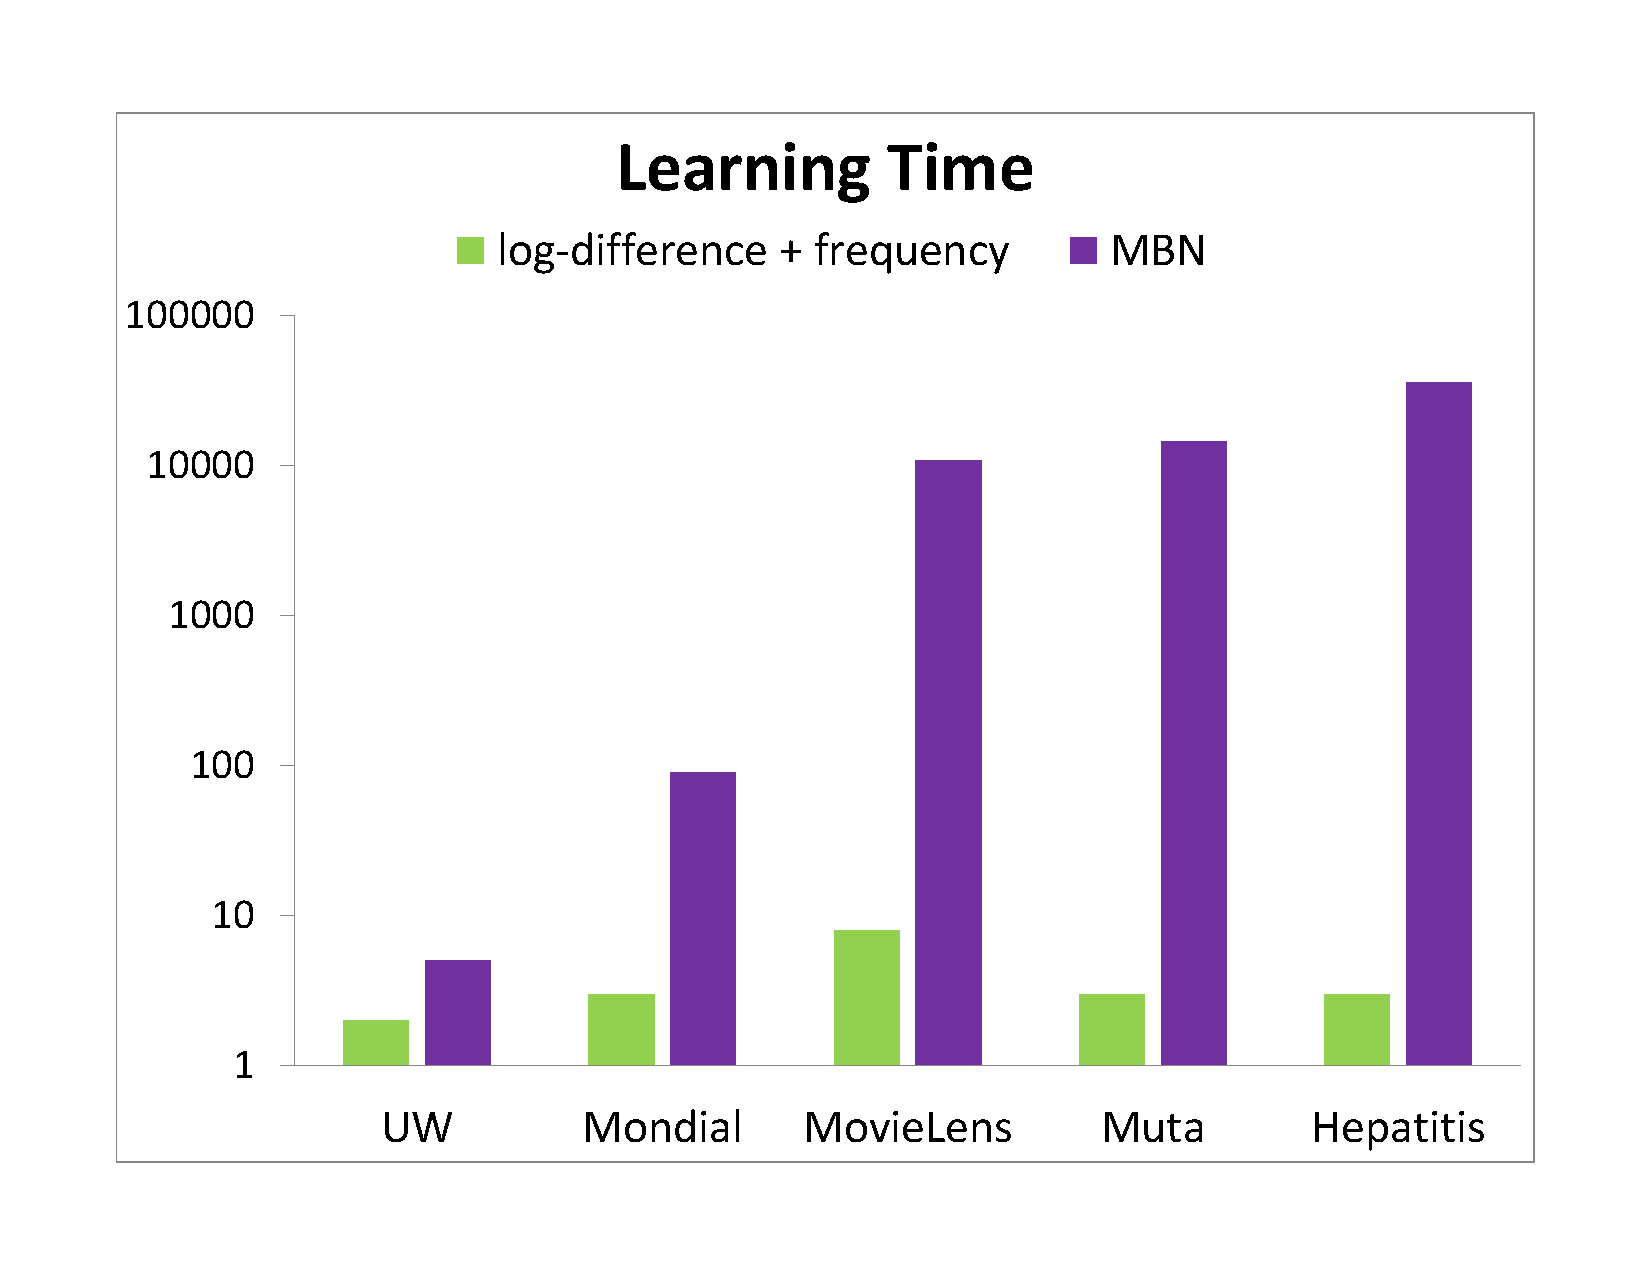
\includegraphics[height=0.5\textheight]{learning_time}
\caption{Predictive Performance averaged over all five benchmark databases. With Bayes net parameters, the frequency model performs better than the count model in terms of likelihood ratios. 
%General weight learning is much slower than Bayes net parameter learning; note that learning times are plotted on a logarithmic scale.
%\fixneeded{Expand ``Prob'' to ``Probability''.}
%\fixneeded{The 2D bars are much better---but they are still darker at the bottom.}
}
\label{fig:summarize}
\end{center}
\end{figure}

\point{Learning Times}
Table~\ref{table:learn-times} shows run time results for structure and parameter learning. We see \keypoint{clear scalability advantages for the maximum likelihood conditional probability estimates used in the Bayes approach}: they take seconds to compute, whereas Alchemy weight optimization requires as much as 10 hours in the worst case (Hepatitis). 

\begin{table}[t]
\caption{Parameter learning times for MBN and Bayes net methods. 
We characterize each database by its counts of ground atoms, tuples,
and Bayes net parameters, and its time for structure learning. The Bayes net
parameter count is the number of family configurations in the Bayes
net.}
\begin{center}
\begin{tabular}{|l r r c c|r c|}
\hline
Dataset & Literals~ & Tuples~  & Parms. & Struct. & MBN~ & Bayes \\
& ($\times 1000$) & ($\times 1000$) & ($\times 10$) & (s) & {(s)\quad} & (s) \\\hline
UW & {3\quad} & {1\quad} & 12 & 36 & 5~~ & \bf{2} \\
Mondial & {2\quad} & {1\quad}  & 58 & 12 & 90~~ & \bf{3}\\
MovieLens & {170\quad} & {82\quad} & 33 & 72 & 10800~~ & \bf{8}\\
Mutagenesis & {35\quad} & {15\quad} & 88 & 30 & 14400~~ & \bf{3}\\
Hepatitis & {71\quad} & {15\quad} & 79 & 24 & 36000~~ & \bf{3}\\\hline
\end{tabular}
\end{center}
\label{table:learn-times}
\end{table}


\point{Summary} 
The findings from this section and the previous one support our claim that balancing the scales of feature functions is important for using Bayes net parameters in a log-linear model. The combination of  transformed BN parameters +feature frequencies  is as predictively accurate as using feature counts with optimized general weights.
While the Bayes net log-linear model is comparable in accuracy, its parameters can be learned much faster than general log-linear weight learning.
%

 
 





 

\section{Conclusion and Future Work} 
\label{sec:conclusion}

Our log-linear equation with relevant feature frequencies appears to be a principled, fast-to-learn, and accurate model for relational prediction with Bayes nets.




\section*{Acknowledgements} This work was supported by Discovery Grants to Oliver Schulte from the Natural Science and Engineering Council of Canada. Zhensong Qian was supported by a grant from the China Scholarship Council. A preliminary version of this paper was presented at the StarAI 2012 workshop. We are indebted to workshop reviewers and participants for helpful comments.
\bibliographystyle{plain}
\bibliography{master}
\end{document}
